% -*- TeX:de -*-
\NeedsTeXFormat{LaTeX2e}
\documentclass[12pt,a4paper]{article}
\usepackage[german]{babel} % german text
\usepackage[DIV12]{typearea} % size of printable area
\usepackage[T1]{fontenc} % font encoding
%\usepackage[latin1]{inputenc} % most likely on Windows
\usepackage[utf8]{inputenc} % probably on Linux
\usepackage{multicol}

% PLOTTING
\usepackage{pgfplots} 
\usepackage{pgfplotstable}
\usepackage{url}
\usepackage{graphicx} % to include images
\usepackage{tikz}
\usepackage{subfigure} % for creating subfigures
\usepackage{amsmath} % a bunch of symbols
\usepackage{amssymb} % even more symbols
\usepackage{booktabs} % pretty tables
\usepackage{makecell} % multi row table heading

% a floating environment for circuits
\usepackage{float}
\usepackage{caption}

%\newfloat{circuit}{tbph}{circuits}
%\floatname{circuit}{Schaltplan}

% a floating environment for diagrams
%\newfloat{diagram}{tbph}{diagrams}
%\floatname{diagram}{Diagramm}

\selectlanguage{german} % use german

\begin{document}

%%%%%%% DECKBLATT %%%%%%%
\thispagestyle{empty}
			\begin{center}
			\Large{Fakultät für Physik}\\
			\end{center}
\begin{verbatim}


\end{verbatim}
							%Eintrag des Wintersemesters
			\begin{center}
			\textbf{\LARGE SS 14}
			\end{center}
\begin{verbatim}


\end{verbatim}
			\begin{center}
			\textbf{\LARGE{Physikalisches Praktikum\\ für das Bachelorstudium}}
			\end{center}
\begin{verbatim}




\end{verbatim}

			\begin{center}
			\textbf{\LARGE{PROTOKOLL}}
			\end{center}
			
\begin{verbatim}

\end{verbatim}

			\begin{flushleft}
			\textbf{\Large{Experiment (Nr., Titel):}}\\
							%Experiment Nr. und Titel statt den Punkten eintragen
			\LARGE{PS08 Halbleiter 2 - Transistoren und Verstärkungsschaltungen}	
			\end{flushleft}

\begin{verbatim}

\end{verbatim}	
							%Eintragen des Abgabedatums, oder des Erstelldatums des Protokolls
			\begin{flushleft}
			\textbf{\Large{Datum:}} \Large{03.04.2014}
			\end{flushleft}
			
\begin{verbatim}
\end{verbatim}
							%Namen der Protokollschreiber
		\begin{flushleft}
			\textbf{\Large{Namen:}} \Large{Patrick Braun, Johannes Kurz}
			\end{flushleft}

\begin{verbatim}


\end{verbatim}
							%Kurstag und Gruppennummer, zb. Fr/5
			\begin{flushleft}
			\textbf{\Large{Kurstag/Gruppe:}} \Large{DO/4}
			\end{flushleft}

\begin{verbatim}

\end{verbatim}
							%Name des Betreuers, das Praktikum betreute.
			\begin{flushleft}
			\LARGE{\textbf{Betreuer:}}	\Large{Johanna Akbarzadeh}	
			\end{flushleft}

%%%%%%% DECKBLATT ENDE %%%%%%%
\pagebreak
\setlength{\columnsep}{20pt}
\begin{multicols}{2}

%%%%%%%%%%%%%%%%%%%%%%%%%%%%%%%%%%%%%%%%%%%%%%%%

%\begin{figure}[H]
%	\centering
%	\includegraphics[scale=0.35]{./data/beugung.png}
%	\caption{Beugungsmuster Einzelspalt (echtes Foto; schwarz durch weiß ersetzt)}
%	\label{fig:beugungsmuster}
%\end{figure}


%\begin{figure}[H]
%	\centering
%	\pgfplotstabletypeset[
%			columns={abstand, n},
%			col sep=&,
%			columns/abstand/.style={precision=2, zerofill, column name=\makecell{$Abstand$\\$(\pm 0.05)[mm]$} }, 
%			columns/n/.style={column name=\makecell{$n$\\$(Ordnung)$}, precision=0},
%			every head row/.style={before row=\hline,after row=\hline\hline},
%			every last row/.style={after row=\hline},
%			every first column/.style={column type/.add={|}{} },
%			every last column/.style={column type/.add={}{|} }
%			]{
%			abstand & n
%			12.9 & 1
%			24.45 & 2
%			37.40 & 3
%			49.35& 4
%			62.45 & 5
%			74.45 & 6
%			87.45 & 7
%			100.25 & 8
%			
%			}
%	\caption{Messwerte Einzelspalt}
%	\label{tab:werte_einzelspalt}
%\end{figure}


%%%%%%%%%%%%%%%%%%%%%%%%%%%%%%%%%%%%%%%%%%%%%%%%
%%%%%%%%%%%%%%%%%%%%%%%%%%%%%%%%%%%%%%%%%%%%%%%%
\noindent In PS08 wird die Funktionsweise und das Verhalten von Transistoren untersucht, sowie konkret diverse Kennlinien einerseits eines bipolaren Transistors und andererseits eines Feldeffekttransistors gemessen und dargestellt.\\

Ein Transistor ist ein Bauteil in dem eine Eingangsspannung ein Ausgangssignal steuert, also ein steuerbarer (genauer "übertragender") Widerstand. Sowohl als elektronische Bauelemente (wie zum Beispiel in den Messungen dieser Experimente) wie auch innerhalb von integrated circuits oder Mikrochips, in Mengen bis zu einer Größenordnung von $10^{10}$ Transistoren pro Chip, sind verschiedene Typen ausgeführt.\\



\section{Bipolartransistor}
\subsection{Grundlagen}
In bipolaren Transistoren sind sowohl positive als auch negative Ladungsträger am Ladungstransport beteiligt (daher der Name).\\

Ein Transistor ist aus 3 Schichten aufgebaut, der Basis $B$, dem Emitter $E$ und dem Kollektor $C$, jeweils mit einem Anschluss. Man unterscheidet, je nach der Dotierung der Außen- bzw der Innenschicht zwischen npn- und pnp-Transistoren, abgesehen von der Polarität der Spannungen und dem Vorzeichen der Ladungen funktionieren diese identisch.\\
Durch diesen Aufbau ergibt sich eine Situation, ähnlich 2 Dioden, die sich eine gemeinsame Anode (npn) oder Kathode (pnp) teilen (die Basis), wobei Emitter und Kollektor unterschiedlich stark dotiert sind (Abb \ref{fig:bipolar_transistor_skizze}).

\begin{figure}[H]
	\centering
	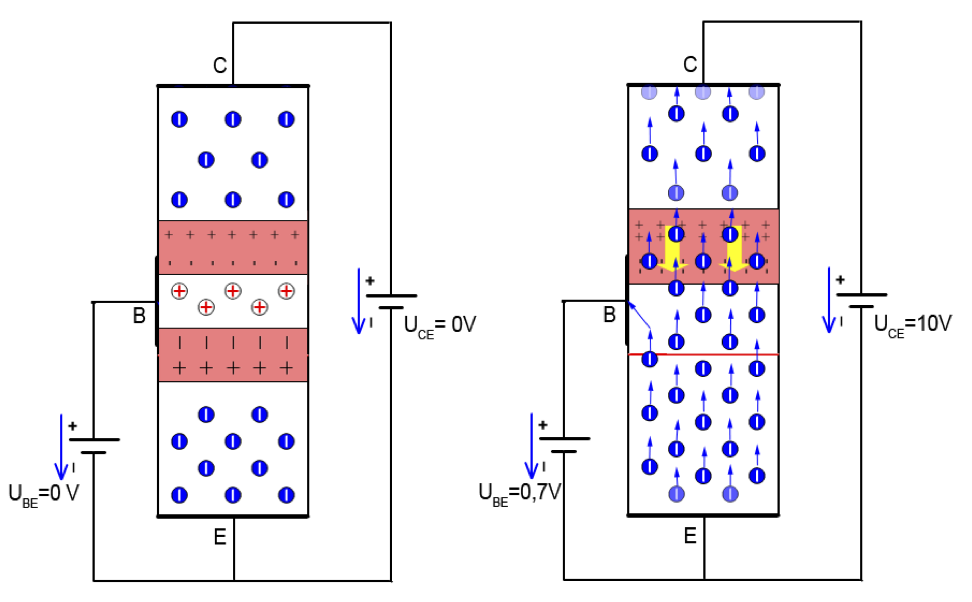
\includegraphics[scale=0.55]{./data/bipolar_transistor_skizze.png}
	\caption{Funktionsweise eines bipolaren npn-Transistors}
	\label{fig:bipolar_transistor_skizze}
\end{figure}

Am linken Teil der Skizze liegt keine Spannung $U_{BE}$ an der Base-Emitter-Schleife an. Beide Sperrschichten im Transistor sind geschlossen und kein Strom fließt.\\
Sobald eine Spannung an diesem Kreis anliegt, verschwindet die Sperrschicht Base-Emitter (wie bei einer Diode). Elektronen aus dem Emitter gelangen in die Basis (und Löcher aus der Basis pflanzen sich umgekehrt fort - daher "bipolar").\\
Hier kommt zum tragen, dass die Basis sehr dünn ist und schwach dotiert. Das führt dazu, dass nur ein sehr kleiner Teil der Ladungen ($<1\%$) mit den Löchern der Basis rekombiniert und zu einem Basisstrom führt. Der überwiegende Teil der Ladungen geht über die dünne Basisschicht, angezogen vom großen Potential des Kollektors in die Schleife zwischen Kollektor und Emitter, zur Spannungsquelle $U_{CE}$.\\
Im Fall einer Verstärkung beispielsweise lässt sich so also durch ein Signal $U_{BE}$, mit kleinen Amplituden, der Spannungsverlauf in $U_{CE}$, mit wesentlich höheren Spannungen, steuern.\\


\subsection{Versuchsaufbau}

In diesem Versuch werden verschiedene Kennlinien eines bipolaren Transistors ("BC 548B", npn) vermessen. Dazu wird das RC2000-System verwendet, ein Modulsystem, bestehend aus Software zur Messung und Darstellung der Daten, einem Steckbrett mit Anschlüssen für Untermodule. Hier werden ein Modul mit fest verdrahteten Anschlüssen, passend zum Vermessen von Transistoren, eine Gleichspannungsquelle, ein Wavegenerator und dazu ein Verstärkermodul verwendet.\\
Mit dem RC2000 können gleichzeitig 2 Spannungen gemessen werden, wobei eine vom System direkt gesteuert wird und in einem definierten Bereich einen Sweep durchführt, um eben eine Kennlinie zu messen. Ströme werden indirekt gemessen, indem die Software aus einer Spannungsmessung an einem bekannten Widerstand den Strom direkt berechnet.\\





\subsection{Resultate}


\subsection{Diskussion}

%%%%%%%%%%%%%%%%%%%%%%%%%%%%%%%%%%%%%%%%%%%%%%%%
%%%%%%%%%%%%%%%%%%%%%%%%%%%%%%%%%%%%%%%%%%%%%%%%
\section{Feldeffekt-Transistor (FET)}
\subsection{Grundlagen}
Auch ein FET ist ein Widerstand, der durch eine (geringe) Spannung gesteuert werden kann, und damit eben als Schalter für einen Leiter oder eben als signalverstärkendes Bauteil verwendet werden kann.\\
Wie der bipolare Transistor hat auch der FET 3 Anschlüsse, die Funktionsweise ist aber komplett verschieden:\\
Der Widerstand einer Leitung (deren Eingang "Source $S$" und Ausgang "Drain $D$" genannt werden) wird durch ein transversales elektrisches Feld erzeugt. Dieses wird wiederum von einer kleinen Steuerspannung am "Gate $G$"-Anschluss gesteuert (

%\begin{figure}[H]
%	\centering
%	\includegraphics[scale=0.35]{./data/beugung.png}
%	\caption{Beugungsmuster Einzelspalt (echtes Foto; schwarz durch weiß ersetzt)}
%	\label{fig:beugungsmuster}
%\end{figure}


\subsection{Resultate}


\subsection{Diskussion}
In Abbildung \ref{fig:eingangskennlinien_fet} ist die Eingangskennlinie des Feld-Effekt-Transistors (FET) zu sehen.
Diese weicht kaum vom Verhalten des normalen Transistors ab.\\
Die Schwierigkeit bei der Ermittlung der Eingangskennlinie des FET war die passenden Einstellungen für die Output Ramp zu finden. Von 0V-2V brachte den gewünschten Bereich.\\ 
Des weiteren war nicht Immer klar welche Spannungen gemessen werden sollen, da die Bezeichnungen in [1] nicht sofort eingeordnet werden konnten.\\
\\
Die J-FET-Ausgangskennlinie ist ersichtlich in Abbildung \ref{fig:ausgangskennlinienfeld_fet} ersichtlich. Gemessen bei 0V, -1V, -2V und -2.5V.\\
Die Ergebnisse der Ausgangskennlinien stimmen im Verhalten mit den in [1](p. 21) überein, jedoch ist der Anstieg im ohmschen Bereich stärker ausgeprägt. Die negativen Spannungen sind nötig da der verwendete FET beim Anlegen der Spannung den Source-Drain Kanal freilegt und somit einen Teil oder die ganze Sperrschicht leitend wird.



\section{Quellen}
$[1]$ Anleitung, \url{http://www.univie.ac.at/anfpra/neu1/ps/ps8/PS8.pdf}\\

\end{multicols}
\section{Anhang}

\begin{figure}[H]
	\centering
	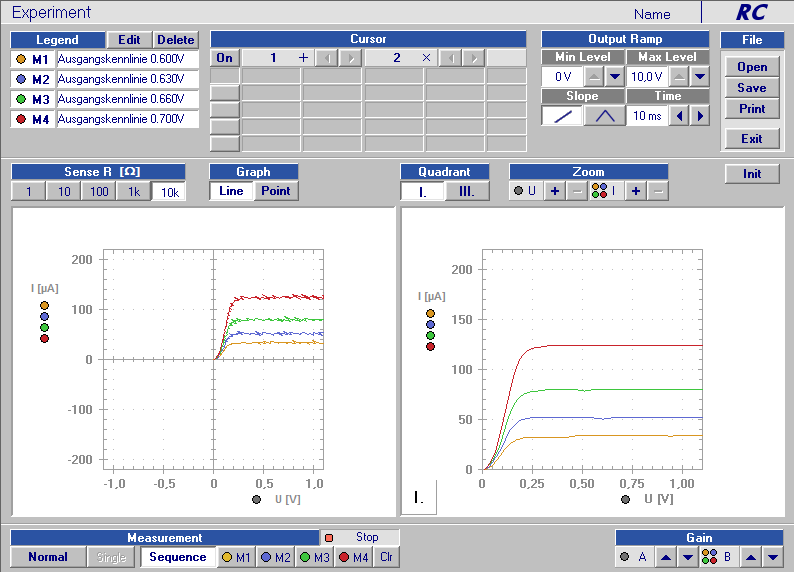
\includegraphics[scale=0.45]{./data/Braun_Kurz_PS8/Ausgangskennlinienfeld.png}
	\caption{Ausgangskennlinienfeld für die Gleichstromverstärkung}
	\label{fig:ausgangskennlinienfeld}
\end{figure}

\begin{figure}[H]
	\centering
	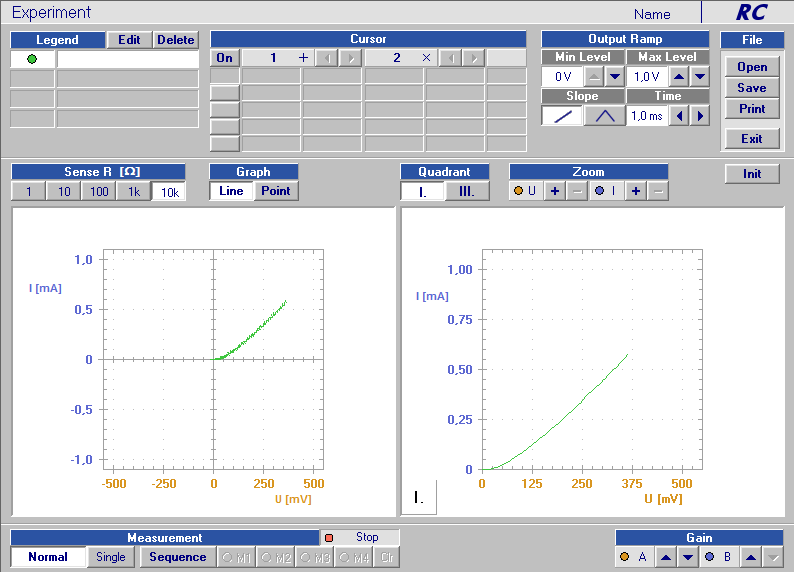
\includegraphics[scale=0.45]{./data/Braun_Kurz_PS8/Gleichstromverstaerkung.png}
	\caption{Eingangskennlinie für die Gleichstromverstärkung}
	\label{fig:eingangsskennlinien}
\end{figure}

\begin{figure}[H]
	\centering
	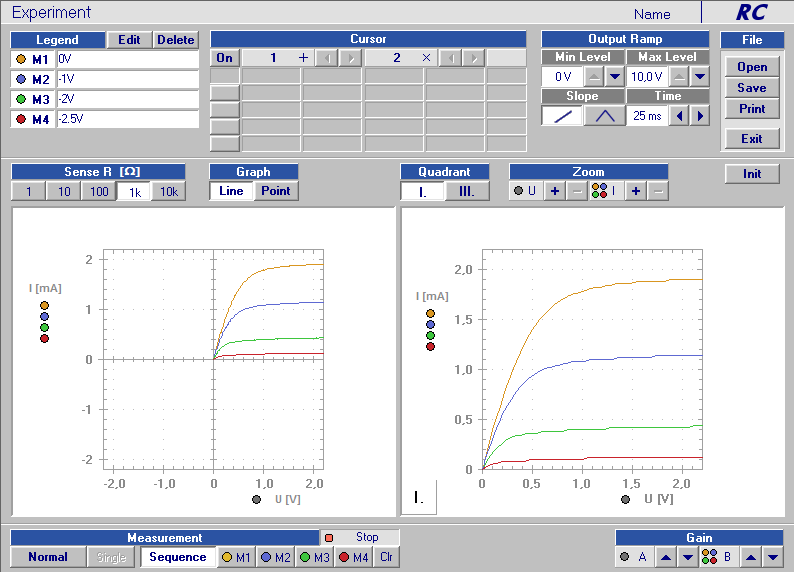
\includegraphics[scale=0.45]{./data/Braun_Kurz_PS8/FET_Ausgangskennlinien.png}
	\caption{Ausgangskennlinienfeld eines Feldeffekt-Transistors}
	\label{fig:ausgangskennlinienfeld_fet}
\end{figure}

\begin{figure}[H]
	\centering
	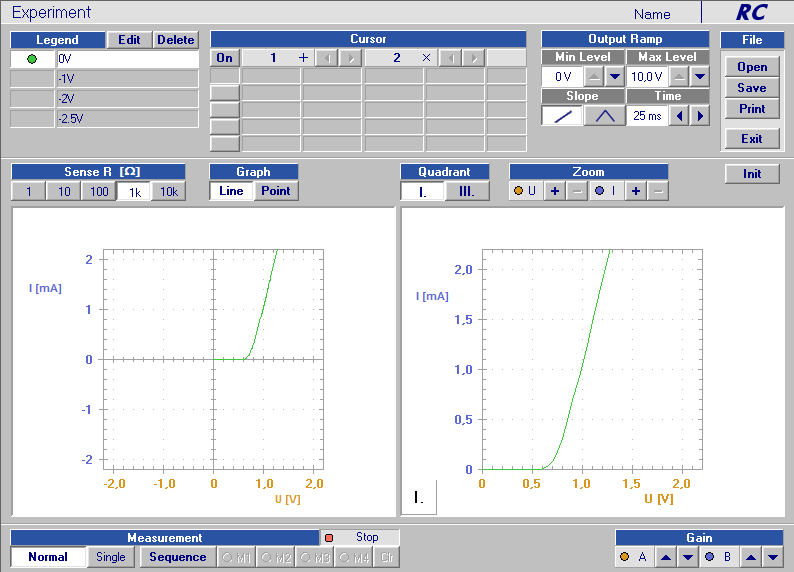
\includegraphics[scale=0.45]{./data/Braun_Kurz_PS8/FET_Eingangskennlinie.png}
	\caption{Eingangskennlinie eines Feldeffekt-Transistors}
	\label{fig:eingangskennlinien_fet}
\end{figure}

\begin{figure}[H]
	\centering
	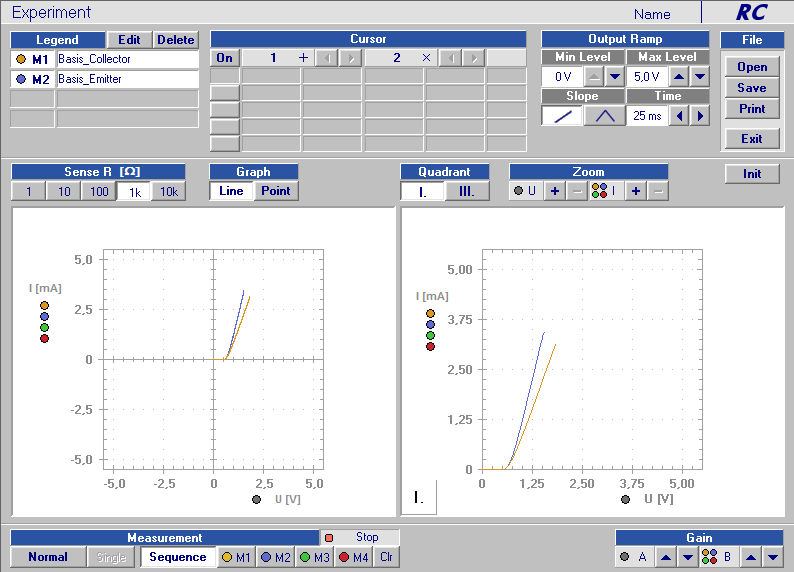
\includegraphics[scale=0.45]{./data/Braun_Kurz_PS8/Kennlinien_Emitter_Collector.png}
	\caption{Kennlinie zwischen Base und Emittier sowie Base und Collector}
	\label{fig:kenn_emit_coll}
\end{figure}

\begin{figure}[H]
	\centering
	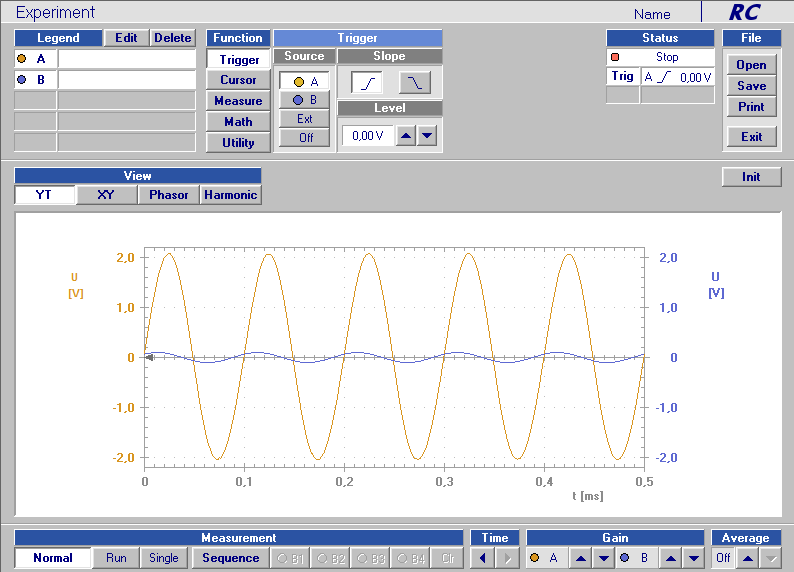
\includegraphics[scale=0.45]{./data/Braun_Kurz_PS8/Kleinsignalverstaerkung.png}
	\caption{Kleinsignalverstärkung}
	\label{fig:kleinsignalverstaerkung}
\end{figure}

\begin{figure}[H]
	\centering
	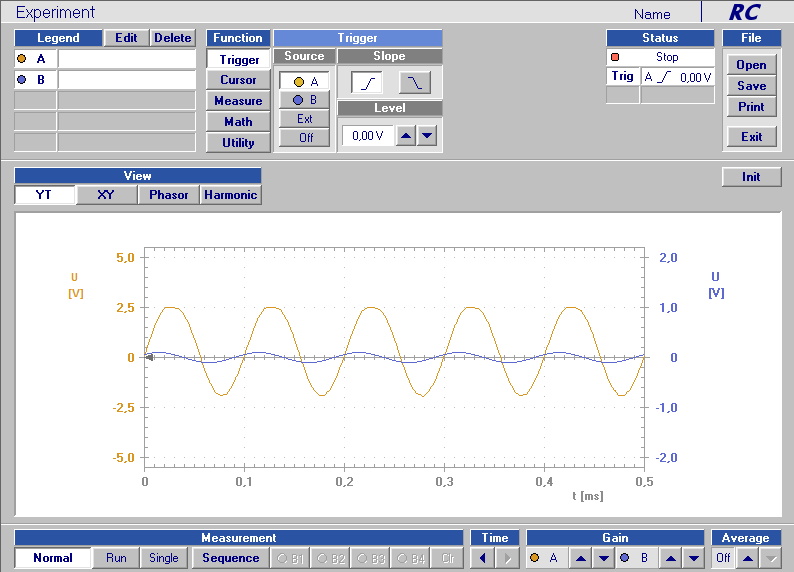
\includegraphics[scale=0.45]{./data/Braun_Kurz_PS8/Kleinsignalverstaerkung_Temp.png}
	\caption{Kleinsignalverstärkung mit erhöhter Temperatur}
	\label{fig:kleinsignalverstaerkung_temp}
\end{figure}

\begin{figure}[H]
	\centering
	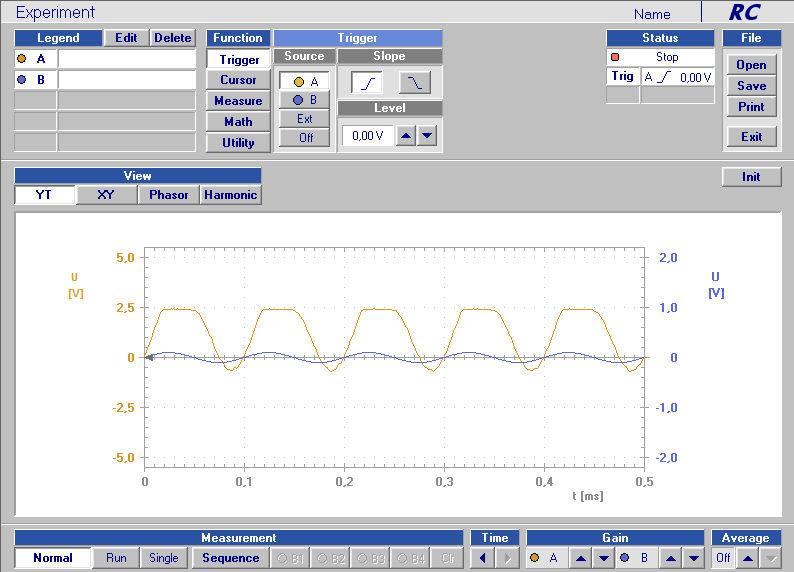
\includegraphics[scale=0.45]{./data/Braun_Kurz_PS8/Kleinsignalverstaerkung_Temp_Cut.png}
	\caption{Kleinsignalverstärkung mit erhöhter Temperatur und sichtbarem Cut}
	\label{fig:kleinsignalverstaerkung_temp_cut}
\end{figure}

\begin{figure}[H]
	\centering
	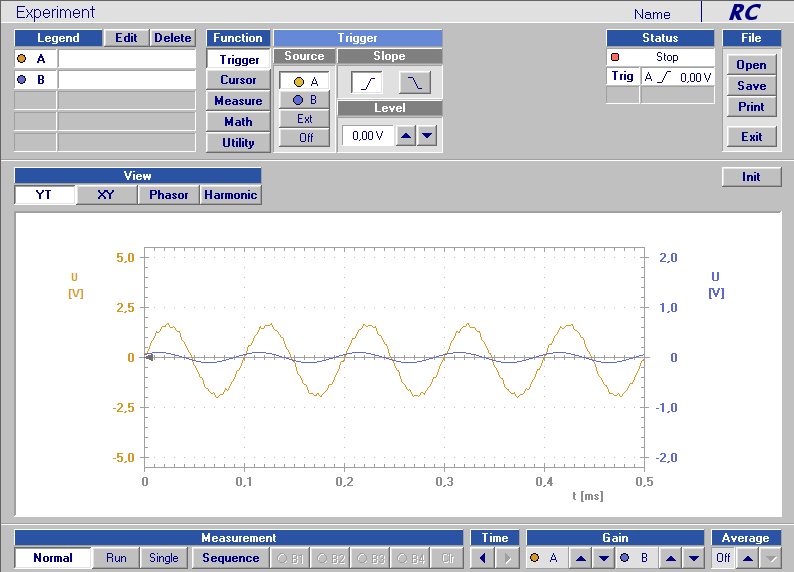
\includegraphics[scale=0.45]{./data/Braun_Kurz_PS8/Kleinsignalverstaerkung_Temp_Gegenspannung.png}
	\caption{Kleinsignalverstärkung mit erhöhter Temperatur und Gegenspannung}
	\label{fig:kleinsignalverstaerkung_temp_gegen}
\end{figure}

\begin{figure}[H]
	\centering
	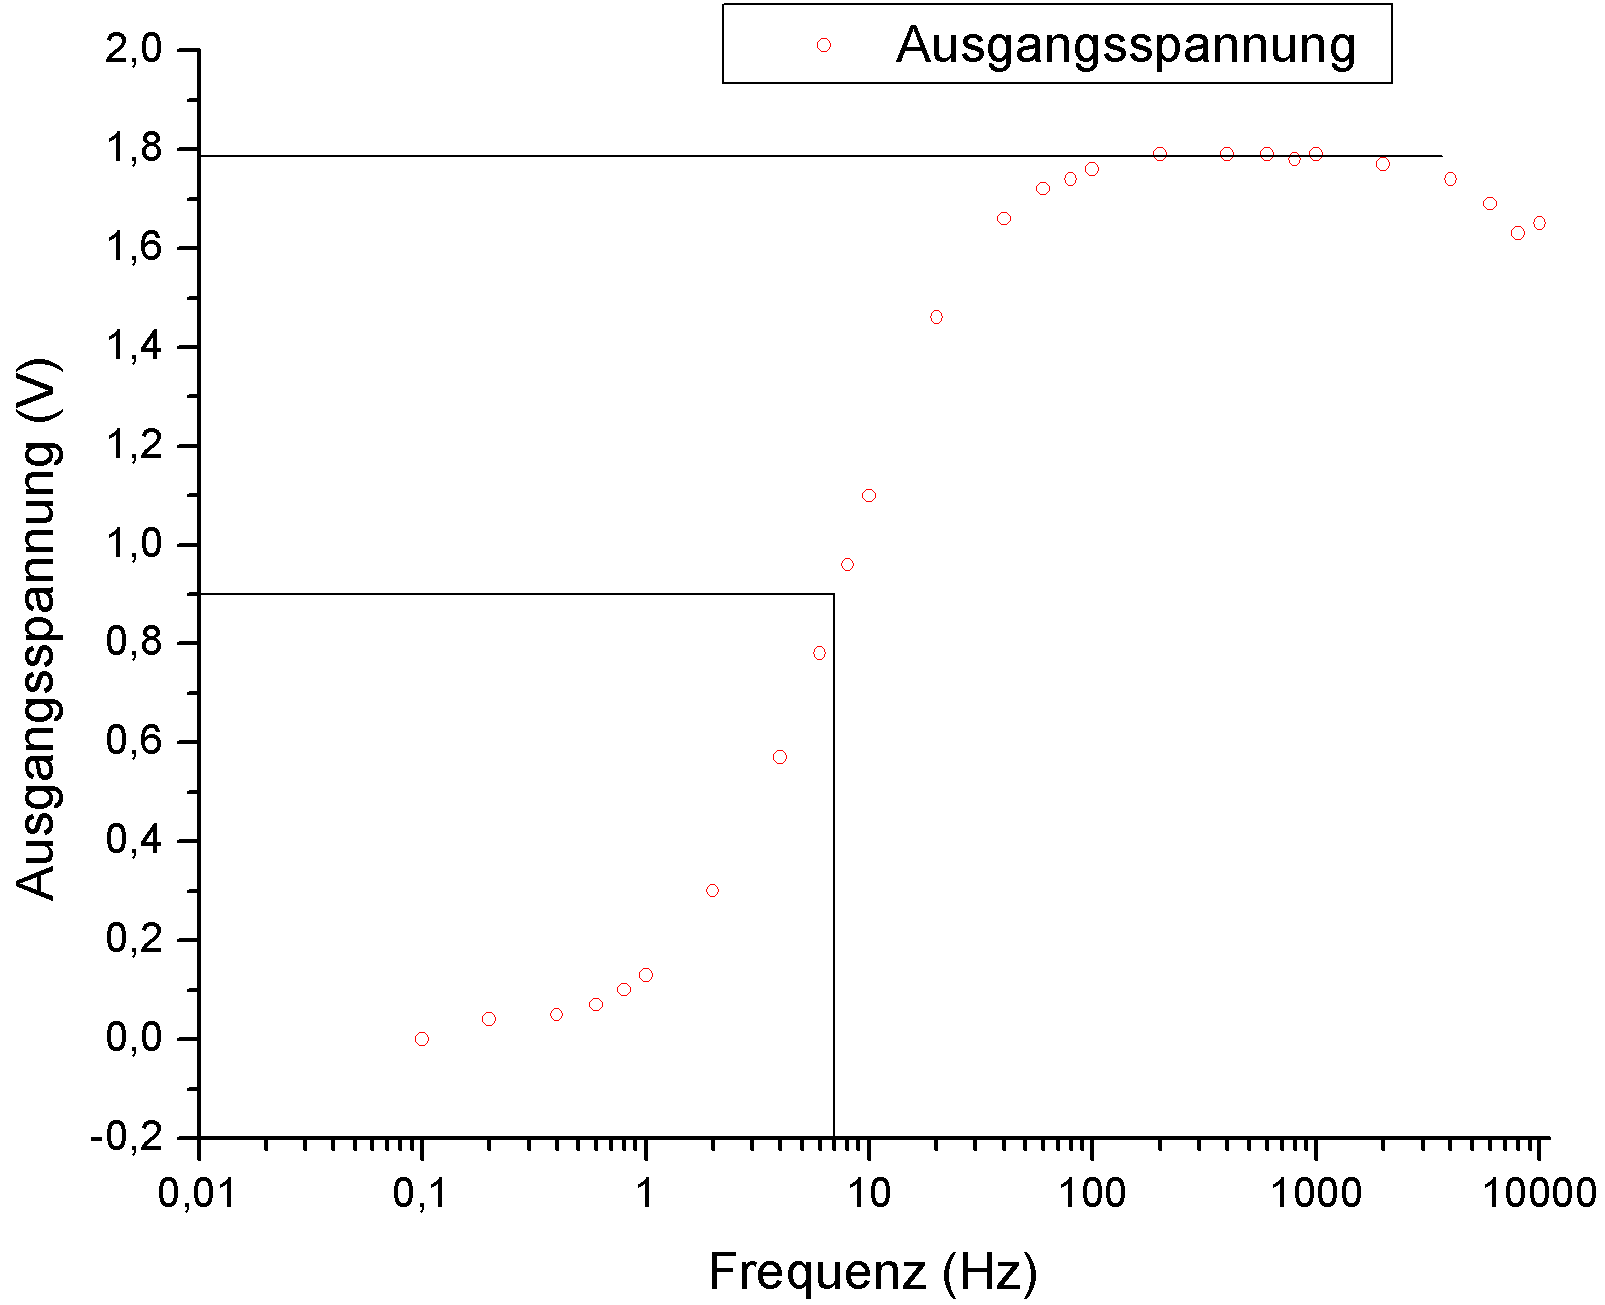
\includegraphics[scale=0.45]{./data/frequenzabhaengigkeit.png}
	\caption{Frequenzabhängigkeit von Verstärkung und Phasenlage}
	\label{fig:frequenzabh}
\end{figure}

\begin{figure}[H]
	\centering
	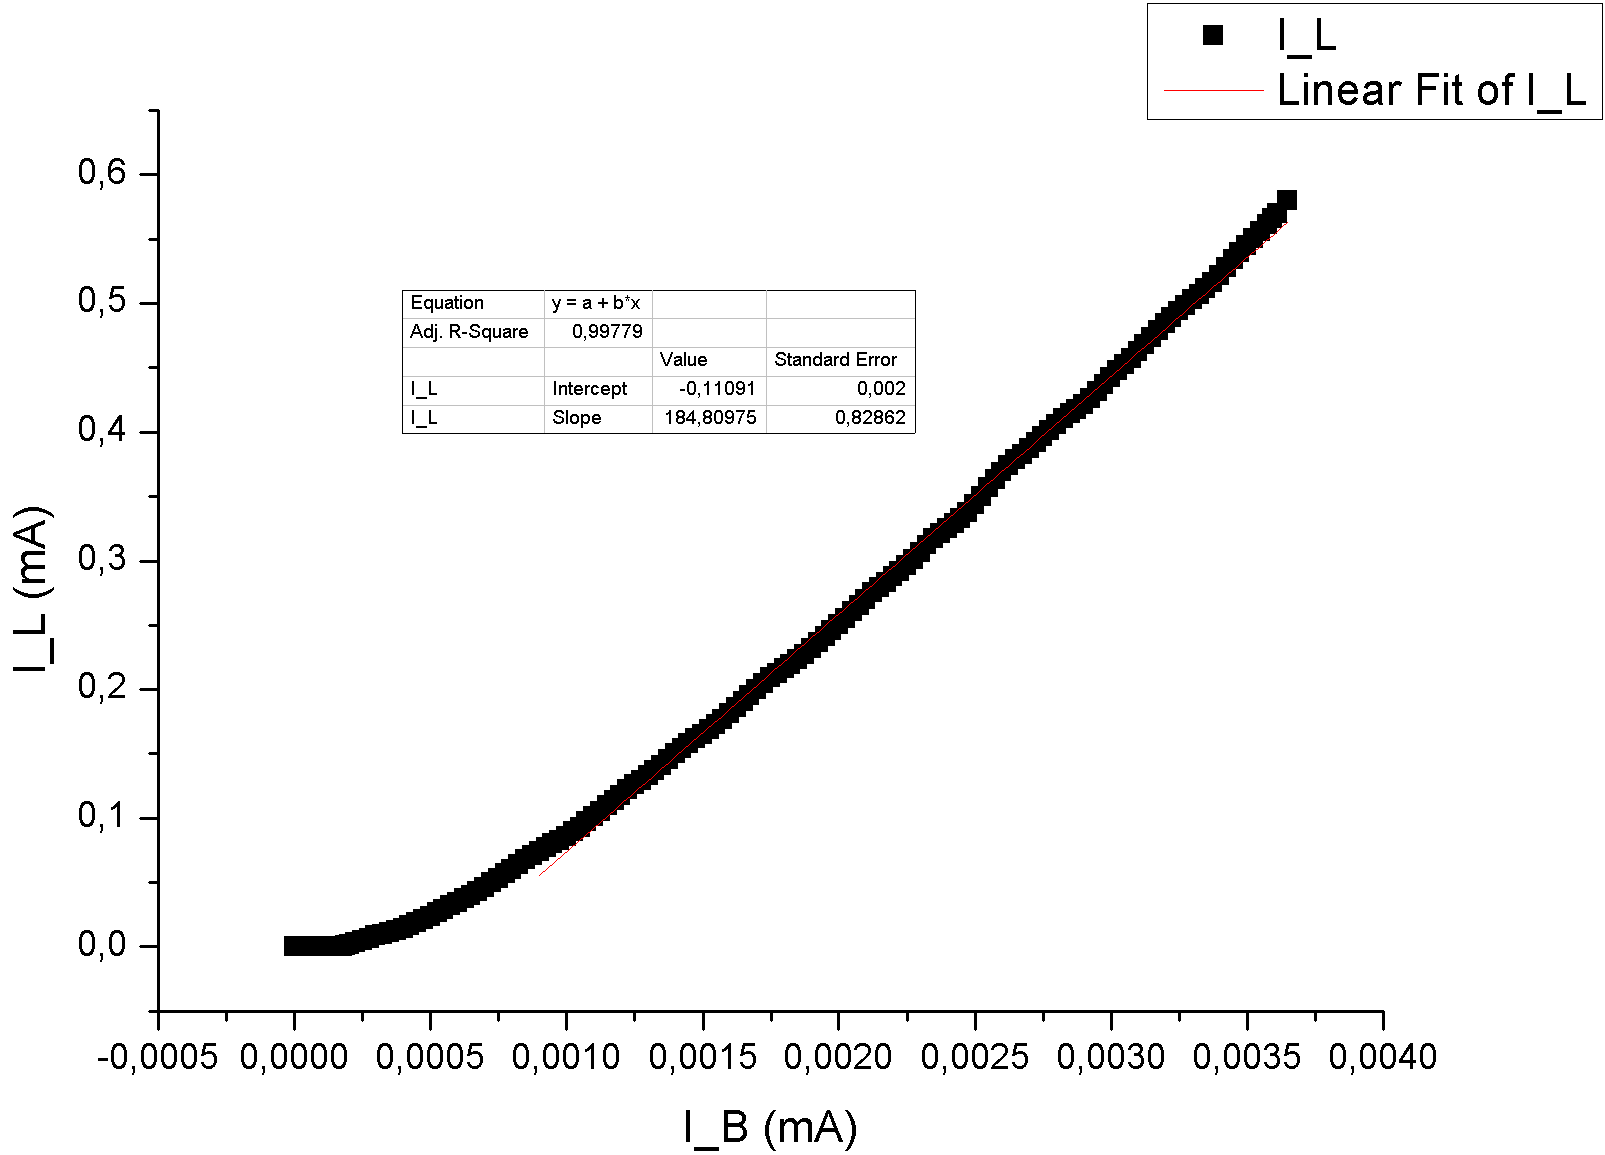
\includegraphics[scale=0.45]{./data/stromverstaerkung.png}
	\caption{Verstärkungsfaktor Gleichstromverstärker}
	\label{fig:verstaerker_faktor}
\end{figure}

\end{document}